\chapter{Auswertung}
In diesem Kapitel werden die Simulationsergebnisse dargestellt und zur Bewertung in Vergleichsparameter zusammengefasst. Für die Simulation werden die in Tabelle \ref{tab:Betriebspara} aufgeführten Betriebsparameter verwendet. Die beiden Topologien werden verglichen, um die beste Lösung zu finden, dabei wird um den Einfluss der Systemdienstleistungen zu berücksichtigen bei einem Phasenversatz von 0° und 30° der Eingangsströme betrachtet. Um die Eingangsströme bei Phasenverschiebung gleich zu halten wird die Ausgangsleistung reduziert um den Faktor $cos(30°)$ . Die Kühlplattentemperatur von 80 °C wird aufgrund der Wahl einer Wasserkühlung für den Demonstrator gewählt.

\begin{table}
	\centering
	\caption{Auflistung der Simulationsbetriebsparameter}
\begin{tabular}{|c|c|}
	\hline
	Netzspannung \gls{Ull} & 617 \si{\volt} \\
	\hline
	Ausgangsspannung \gls{Ua} & 680 V \\
	\hline
	Scheinleistung & 200 kW \\
	\hline
	Phasenverschiebung & 0 / 30 Grad \\
	\hline
	Kühlplattentemperatur & 80 °C \\
	\hline
	Schaltfrequenz & 20 kHz \\
	\hline
\end{tabular}

\label{tab:Betriebspara}
\end{table}


\section{IAF}
Für die Auswertung werden die Simulationen für eine Dauer von einer Sekunde durchgeführt, da zu diesem Zeitpunkt ein eingeschwungener Zustand erreicht ist. Das Temperaturverhalten der Halbleiter ist in Abbildung \ref{fig:iaftemp} dargestellt. Wie in Abbildung \ref{fig:iaftemp} dargestellt, ist die Kühlplattentemperatur als Startpunkt auf 80 °C festgelegt. Die Dioden des Gleichrichters, welche den Hauptstrom führen, sind in grün dargestellt und ändern sich nur minimal aufgrund der Blindleistungsbereitstellung. Die Temperatur beträgt knapp über 120 °C und liegt somit unterhalb der erlaubten Maximaltemperatur von 175 °C \cite{IFAGFF2}. Die Temperatur der T+/- Halbbrücke wird in Pink dargestellt und steigt bei Blindleistungsbereitstellung auf knapp 160 °C und bietet damit 15 °C Abstand zur zulässigen Maximaltemperatur. Die Temperatur des Tiefsetzstellers wird in Rot dargestellt und sinkt aufgrund der Reduzierten Ausgangsleistung bei Blindleistungsbereitstellung.  
\begin{figure}
	\centering
	\subfloat[][]{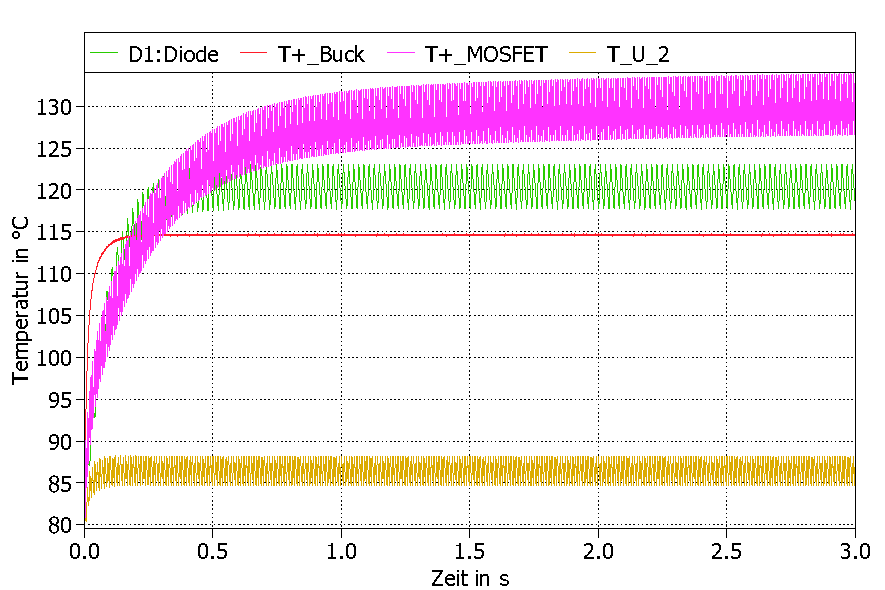
\includegraphics[width=1\linewidth]{content/Grafiken/IAF_Temp_0Grad}}
	\qquad
	\subfloat[][]{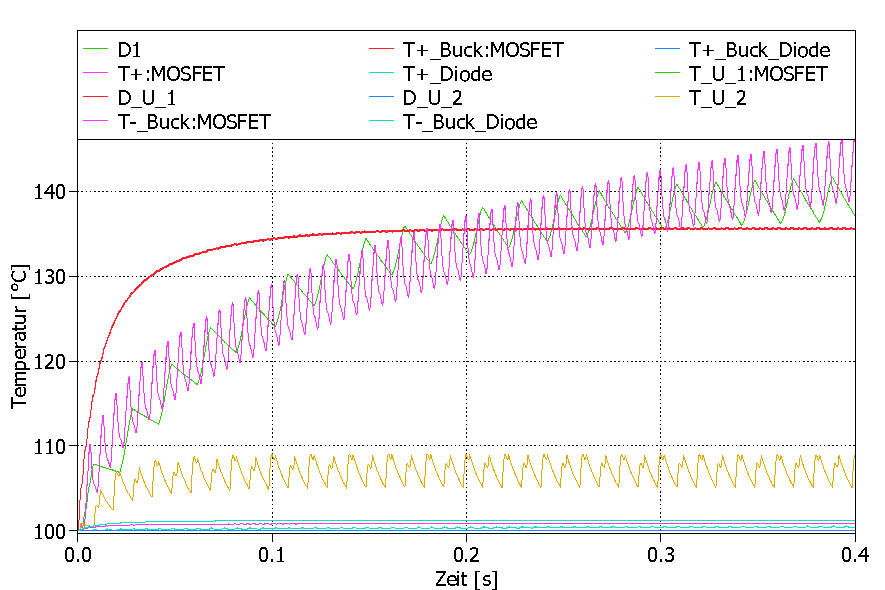
\includegraphics[width=1\linewidth]{content/Grafiken/IAF_Temp_30Grad}}
	\caption{Temperaturverhalten der Halbleiter des IAF ohne (a) und mit (b) Phasenverschiebung}
	\label{fig:iaftemp}
\end{figure}

Die Simulationsergebnisse zeigen den erwarteten Strom- und Spannungsverlauf für die Induktivität mit einer Dreiecksform, siehe Abbildung. \ref{fig:iafacl}. Zusätzlich ist dem Eingangsstrom ein hochfrequenter Anteil überlagert, der durch die Schaltfrequenz des Tiefsetzstellers erklärt werden kann. Außerdem treten beim Schaltvorgang des \gls{IVS} starke Sprünge im Stromverlauf auf, da der Strom in der Induktivität zwischen den Phasen schalten muss.\\
In Abb. \ref{fig:iafacl30grad} wird dieses Problem durch die starken Spannungsunterschiede zwischen den Phasen bei Phasenverschiebung noch verstärkt. Außerdem muss der \gls{IVS} mehr Strom führen und erzeugt dadurch mehr Verlustleistung. Dies ist auch an der Temperatur des in Abb. \ref{fig:iaftemp} dargestellten Kurven erkennbar. Es werden nur die höchsten Temperaturen dargestellt, dies sind die Eingangsdioden, beispielhaft an D1 in grün dargestellt sowie die \gls{MOSFET}s des T+ in pink (der Halbbrücke am \gls{IVS}), der \gls{IVS} in Gelb sowie des Tiefsetzstellers in rot. In (a) ist die Temperatur des IVS unter 90 °C und in (b) durch den höheren Strom aufgrund der Phasenverschiebung deutlich angestiegen. Um den Sinusverlauf im Mittel besser erkennen zu können, ist der Stromverlauf in Abbildung \ref{fig:iafacl30grad} zusätzlich nach einer Tiefpassfilterung dargestellt. Dadurch ist die Phasenverschiebung besser ersichtlich, siehe Verlauf A Filter.
\begin{figure}
	\centering
	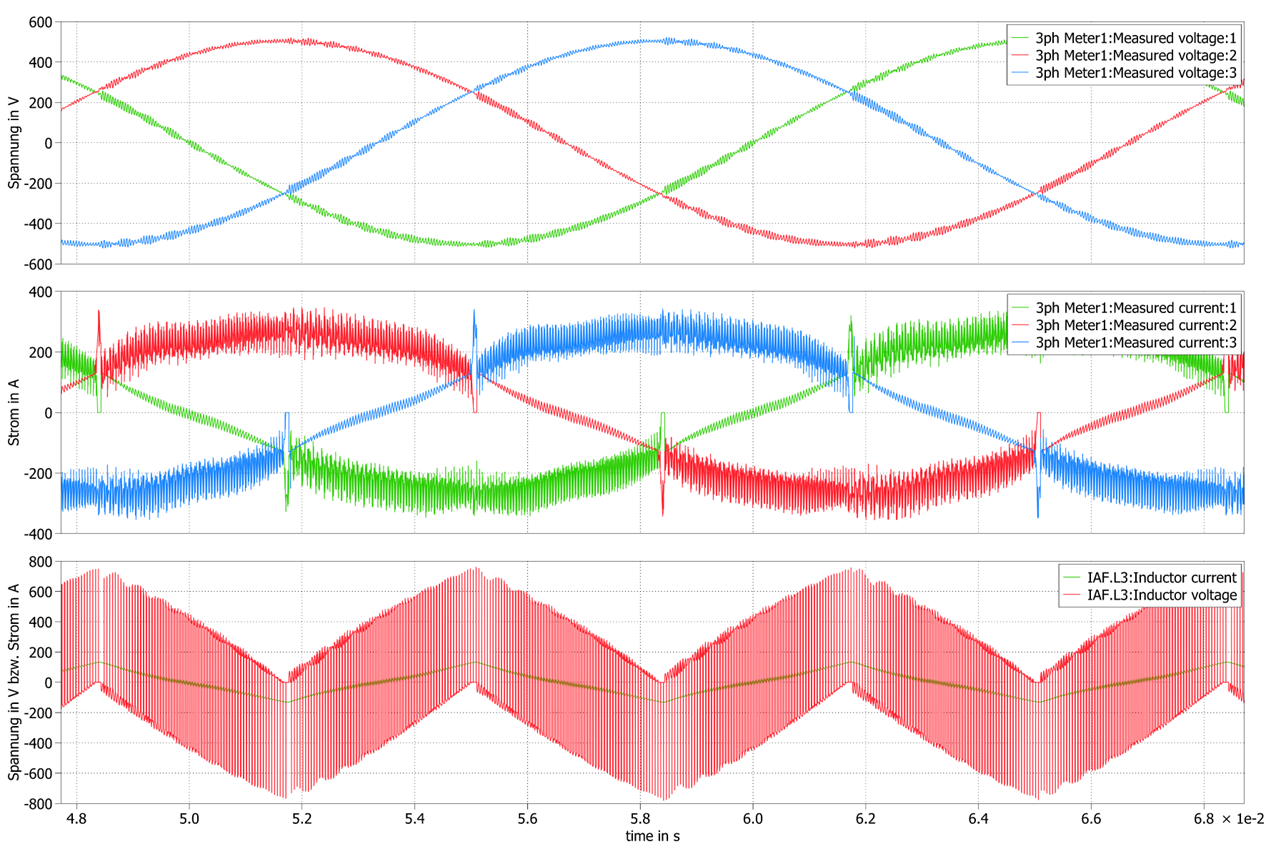
\includegraphics[width=1\linewidth]{content/Grafiken/IAF_AC+L}
	\caption{Simulationsergebnisse des IAF ohne Phasenverschiebung, Eingangsspannung und Ströme, Strom in der IVS Induktivität }
	\label{fig:iafacl}
\end{figure}
\begin{figure}
	\centering
	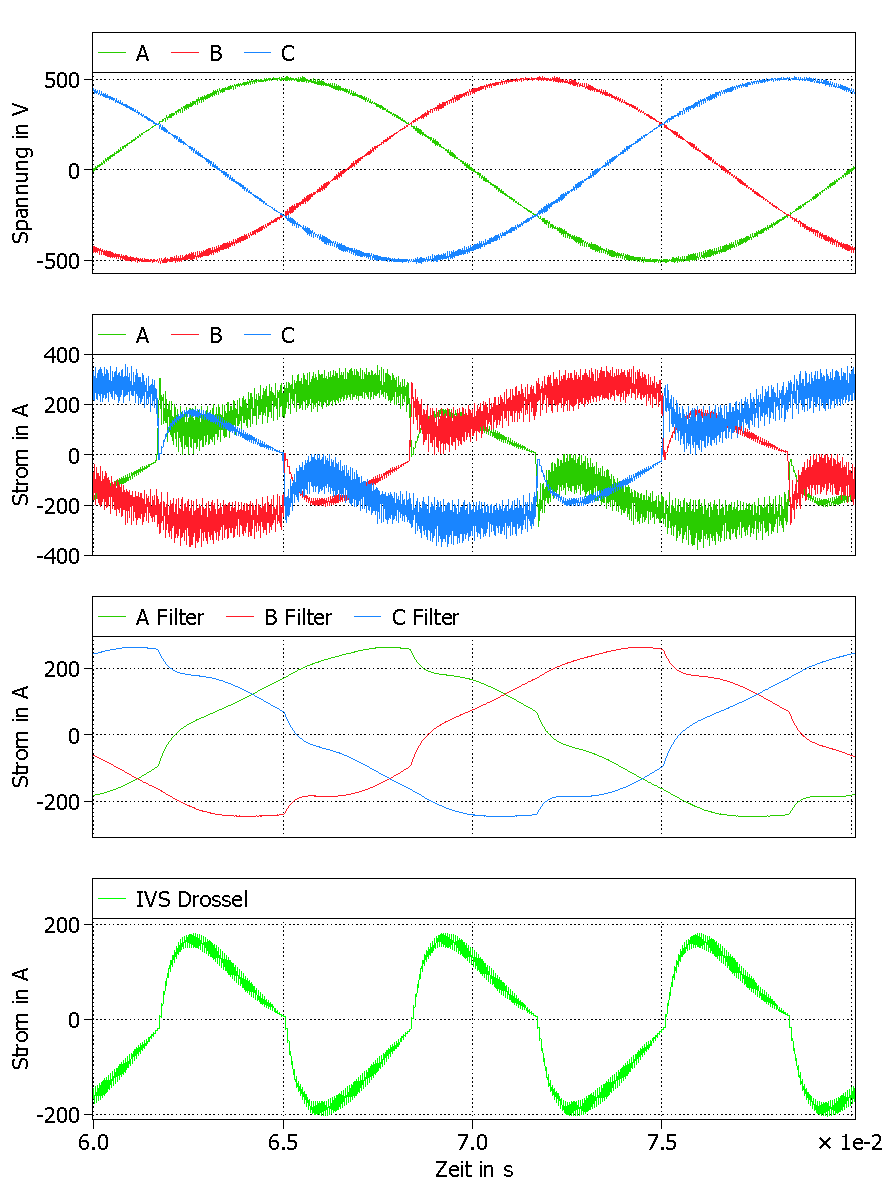
\includegraphics[width=1\linewidth]{content/Grafiken/IAF_AC+L_30Grad}
	\caption{Simulationsergebnisse des IAF bei 30 Grad Phasenverschiebung, Eingangsspannung und Ströme, Strom in der IVS Induktivität }
	\label{fig:iafacl30grad}
\end{figure}
Die Topologie hat aufgrund der Anforderung an Blindleistungsbereitstellung einen Nachteil durch den IVS, da dieser sprunghafte Änderungen des Stromverlaufs verursacht. Diese starken Sprünge führen dazu, dass die THD des Stroms deutlich verschlechtert wird. Die THD liegt bereits ohne Phasenverschiebung bei etwa 15~\%, und mit Phasenverschiebung verdoppelt sich dieser Wert auf etwa 32 \%.  Somit kann der IAF den Anforderungen nur schwer gerecht werden, da weitere Filterstufen benötigt würden. Dies lässt sich auch gut anhand der Arbeit von Schrittwieser et al. sehen. Bei ihrem Prototyp macht der Filter knapp ein Viertel des Volumens aus \cite{IAF99}.

\section{B6-1/3-PWM PFC}
Es zeigt sich, dass der \gls{B6PFC} deutliche Nachteile bei den Induktivitäten und damit bei den Hardwarekosten hat. Die erforderliche dreiphasige Drossel führt dazu, dass der IAF in dieser Kategorie um mehr als 50\% besser abschneidet.
Anders sieht es in den anderen Kategorien aus, wo weniger Kondensatoren benötigt werden. Die erforderliche B6-Schaltung enthält mehr \gls{MOSFET}, dafür aber keine Dioden. Bei der Verlustleistung zeigt sich der klare Vorteil der Topologie bei der Bereitstellung von \gls{SDL}, da sie fast keinen Einfluss auf die Verluste in den Halbleitern hat. Dies lässt sich anhand des Temperaturverhaltens in Abb. \ref{fig:b6temp030grad} bestätigen, durch die Reduzierung der Ausgangsleistung ist die Temperatur im \gls{MOSFET} FET7 des Tiefsetzsteller etwas niedriger, rosa dargestellt. Bei den Halbleitern der B6-Brücke ist praktisch kein Unterschied zu erkennen. Die Eingangsströme sind lediglich durch die Schaltimpulse leicht verrauscht und der Sinusverlauf folgt der Eingangsspannung wie gewünscht, siehe Abbildung \ref{fig:b6acdc0grad}.  Der Stromverlauf weist eine THD von nur etwa 5,8 \% auf.
\begin{figure}
	\centering
	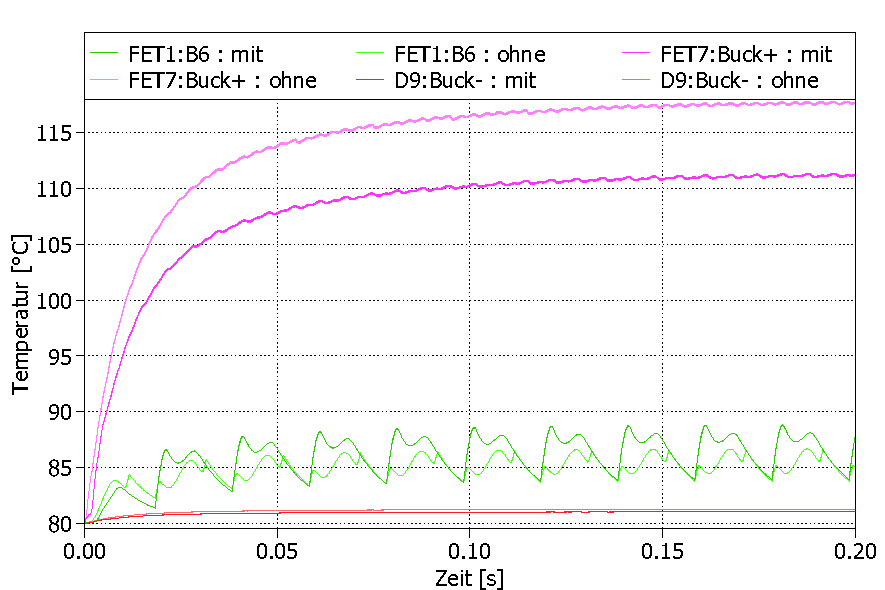
\includegraphics[width=1\linewidth]{content/Grafiken/B6_Temp_0&30Grad}
	\caption{Temperaturverhalten der Halbleiter des B6 mit und ohne Phasenverschiebung}
	\label{fig:b6temp030grad}
\end{figure}

\begin{figure}
	\centering
	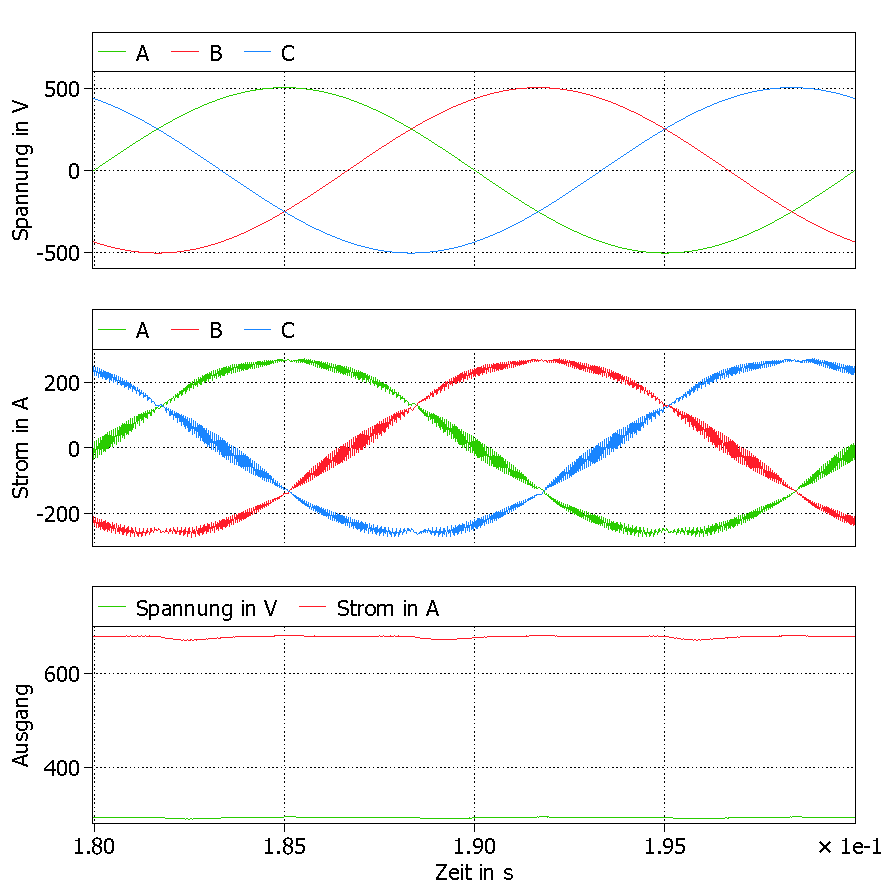
\includegraphics[width=1\linewidth]{content/Grafiken/B6_AC+DC_0Grad}
	\caption{Eingangs- und Ausgangsgrößen ohne Phasenverschiebung}
	\label{fig:b6acdc0grad}
\end{figure}
\pagebreak
Mit einer Phasenverschiebung von 30 Grad sieht das Verhalten ähnlich aus, siehe Abbildung \ref{fig:b6acdc30grad}.  Der Stromverlauf weist eine etwas höhere THD von 7,1 \% auf, die jedoch durch geeignete Filter ausgeglichen werden kann.
\begin{figure}
	\centering
	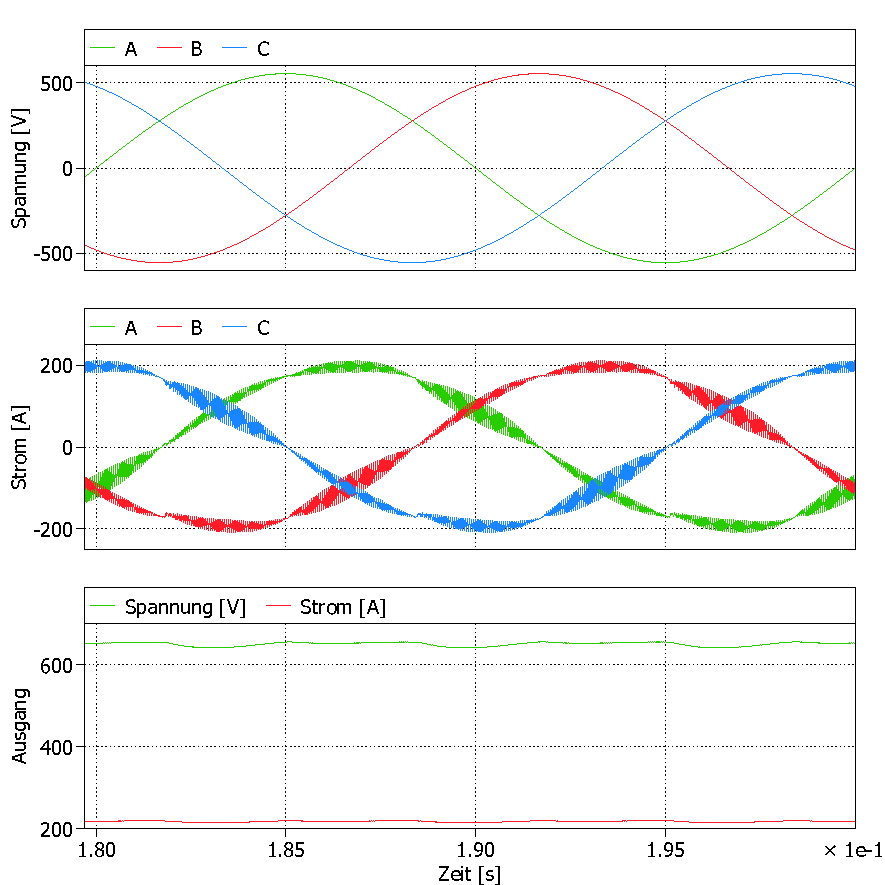
\includegraphics[width=1\linewidth]{content/Grafiken/B6_AC+DC_30Grad}
	\caption{Eingangs- und Ausgangsgrößen mit Phasenverschiebung}
	\label{fig:b6acdc30grad}
\end{figure}

\section{Bewertung}
Die Ergebnisse der Gesamtbewertung sind in Tabelle \ref{tab:Auswertung} aufgeführt. Diese Tabelle enthält Informationen über die Hardware, insbesondere die Induktivitäten, sowie über die Kapazitäten, Halbleiter und Treiber. Zusätzlich werden die Ergebnisse der Simulation anhand der Verlustleistung der Halbleiter bewertet.  Zur Durchführung eines Vergleichs der Kategorien und einer Gesamtbewertung werden die Einzelkategorien zwischen null und eins normiert und mit einem Gewichtungsfaktor summiert. Da die Drosseln einen großen Einfluss haben, werden sie mit 50 Prozent gewichtet. Die Kapazitäten haben nur einen vergleichsweise geringen Einfluss auf die Gesamtsystemkosten und werden daher nur mit fünf Prozent bewertet. Die restlichen 45 Prozent entfallen auf die Halbleiter in Form der Chipfläche (über den RDSON), die Anzahl der Treiber und die Verlustleistung. Die jeweiligen Punkte sind proportional zu erwartenden Systemkosten und Volumen. Daher stellt eine niedrigere Punktzahl eine bessere Bewertung dar. \\
\begin{table}
	\centering
	\caption{Auflistung der Simulationsergebnisse und Bewertung}
	\begin{tabular}{|c|c|c|c|c|}
		\hline
		& Topologie & B6-Buck & \gls{IAF} & Gewichtung: \\
		\hline
		Induktivitäten& L1 Netzinduktivität \si{\micro \henry}& 136 & 1 &  \\
		\hline
		& Gespeicherte Energie J& 17,6 & 0,1 & \\
		\hline
		& L2 DC Induktivität \si{\micro \henry}& 136 & 136 &  \\
		\hline
		& Gespeicherte Energie J& 7,8 & 7,8 &  \\
		\hline
		& L3 IVS Induktivität \si{\micro \henry}& - & 302,2 &  \\
		\hline
		& Gespeicherte Energie J & - & 8,82 & \\
		\hline
		& \textbf{Induktivität normiert:} & \textbf{1}   & \textbf{0,66} & 50\% \\
		\hline
		Kapazitäten & C1 Netzkapazität \si{\micro \farad}& - & 50 &  \\
		\hline
		& C2 DC Ausgang mF& 1 & 1 &  \\
		\hline
		& C3 DC Zwischenkreis \si{\micro \farad}& 25 & 50 &  \\
		\hline
		& \textbf{Kapazität normiert:} & \textbf{0,26} &  \textbf{1} & 5\% \\
		\hline
		Halbleiter & SiC 4 \si{\milli \ohm} & 0 & 2 &  \\
		\hline
		& SiC 2 \si{\milli \ohm} & 10 & 4 &  \\
		\hline
		& SiC 5 \si{\milli \ohm} & 0 & 6 &  \\
		\hline
		& \textbf{MOSFET normiert:} & \textbf{1} &  \textbf{0,64} & 15\% \\
		\hline
		& Dioden & 0 & 6 &  \\
		\hline
		& \textbf{Dioden normiert} & \textbf{0} & \textbf{1} & 5\% \\
		\hline
		Treiber & Treiberanzahl & 8 & 7 &  \\
		\hline
		& \textbf{Treiber normiert:} & \textbf{1} & \textbf{0,88} & 5\% \\
		\hline
		Verluste W & Schaltverluste 30 Grad & 567 & 503 &  \\
		\hline
		& Leitverluste 30 Grad & 254 & 1311 &  \\
		\hline
		& 30 Grad Gewichtung: & 75\% & 75\% &  \\
		\hline
		& Schaltverluste 0 Grad & 554 & 511 &  \\
		\hline
		& Leitverluste 0 Grad & 326 & 748 &  \\
		\hline
		& 0 Grad Gewichtung: & 25\% & 25\% &  \\
		\hline
		& \textbf{Verluste normiert:} &\textbf{0,5} & \textbf{1} & 20\% \\
		\hline
		\textbf{Gesamt} &  & \textbf{0,77} & \textbf{0,74} & \\
		\hline
	\end{tabular}
	\label{tab:Auswertung}
\end{table}